\section{Motivating Example}
\label{motiv:section}

\subsection{Example and Observations}

\begin{figure}[t]
	\centering
	\lstset{
		numbers=left,
		numberstyle= \tiny,
		keywordstyle= \color{blue!70},
		commentstyle= \color{red!50!green!50!blue!50},
		frame=shadowbox,
		rulesepcolor= \color{red!20!green!20!blue!20} ,
		xleftmargin=1.5em,xrightmargin=0em, aboveskip=1em,
		framexleftmargin=1.5em,
                numbersep= 5pt,
		language=Java,
    basicstyle=\scriptsize\ttfamily,
    numberstyle=\scriptsize\ttfamily,
    emphstyle=\bfseries,
                moredelim=**[is][\color{red}]{@}{@},
		escapeinside= {(*@}{@*)}
	}
	\begin{lstlisting}[]
public void toSource(final CodeBuilder cb, int inputSeqNum, Node root) {
	...
(*@{\color{red}{-	String code = toSource(root, sourceMap);}@*)
(*@{\color{cyan}{+	String code = toSource(root, sourceMap, inputSeqNum == 0);}@*)
  if (!code.isEmpty()) {
    cb.append(code);
  } ...
}
//--------------------------------------------------------------------------
(*@@Override@*)
String toSource(Node n) {
 initCompilerOptionsIfTesting();
(*@{\color{red}{-	return toSource(n, null);}@*)
(*@{\color{cyan}{+ 	return toSource(n, null, true);}@*)
}
//--------------------------------------------------------------------------
(*@{\color{red}{- private String toSource(Node n, SourceMap sourceMap) {}@*)
(*@{\color{cyan}{+ private String toSource(Node n, SourceMap sourceMap, boolean firstOutput) {}@*)
	......
  builder.setSourceMapDetailLevel(options.sourceMapDetailLevel);
(*@{\color{red}{-   builder.setTagAsStrict(}@*)
(*@{\color{cyan}{+   builder.setTagAsStrict(firstOutput}@*) && 
		options.getLanguageOut(a) == LanguageMode.ECMASCRIPT5_STRICT);
  builder.setLineLengthThreshold(options.lineLengthThreshold);
	......	
}	
	\end{lstlisting}
        \vspace{-15pt}
        %        \caption{A Multi-statement/Multi-method Bug Fix}
        \caption{Co-Change Fixing Locations for a Fault}
        \vspace{-6pt}
        \label{fig:motiv}
\end{figure}

Let us start with a real-world example on the bug fixes that
require multiple changes to multiple statements in different methods.
Figure~\ref{fig:motiv} shows a bug in Defects4J dataset. The bug
occurred when the method call to \code{setTagAsStrict} did not
consider the first output in its arguments. Therefore, for fixing, a
developer adds a new argument in the method \code{toSource} at line
18, and uses that argument in the method call \code{setTagAsStrict
  (firstOutput,...)} at line 22. Because the method \code{toSource} at
line 17 was changed, the two callers at line 3 of the method
\code{toSource} (line 1) and at line 13 of the method \code{toSource}
(line 11) need to be changed accordingly.

%This is a bug from Defects4J data that has three methods need to be fixed at the same time. The bug is caused by doing the method call $setTagAsStrict$ without checking if it is the first output. To fix this bug, firstly, for the method C, we need to add one more parameter $firstOutput$ for the method call $setTagAsStrict$. Then, for the method A and B, because they call the method C or override the method C, when adding a new parameter in the method C, they all need to do the same thing. We need to add $inputSeqNum == 0$ in method A and add $true$ in method B when calling the method C.

%In this bug, there are multiple statements that need to be fixed and they located in three different methods. Also, when analyzing the co-change information, the method A and method C have been fixed together before in the commit history. 


\begin{figure*}[t]
	\centering
	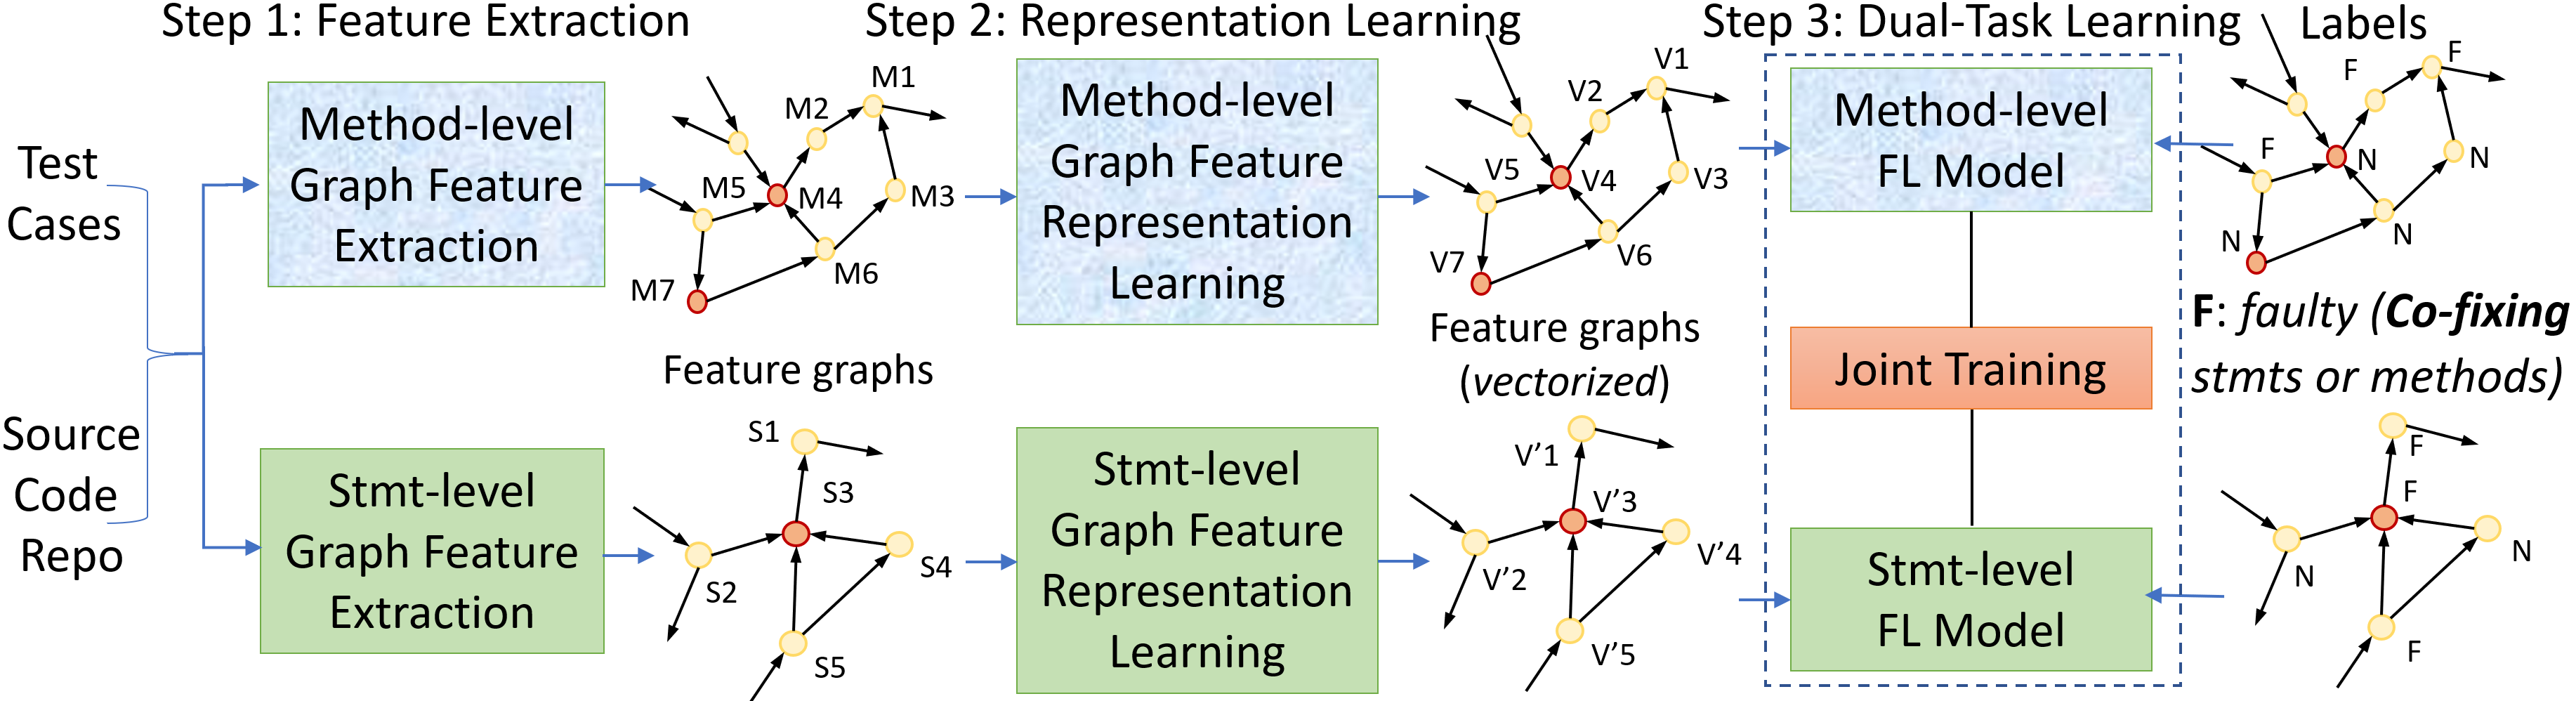
\includegraphics[width=5.65in]{graphs/overview-training-4.png} %5.45
        \vspace{-8pt}
	\caption{{\tool}: Training Process}
        \label{train-overview}
\end{figure*}

\noindent {\bf Observation 1. [Co-Change Fixing Locations]} In this
example, the changes to fix this bug involve multiple faulty
statements that are dependent on one another. Fixing only one of the
faulty statements will not make the program pass the previously
failing test(s). Fixing one buggy statement at a time in the ranked
list returned from an existing FL tool will also not make the program
pass the tests. For an APR model to work, an FL tool needs to point
out all of those faulty statements to be changed in the same fix.

%For effective manually fixing by developers, an FL tool also needs
%point out all faulty statements to be fixed at once. Otherwise, (s)he
%must find the missing locations or waste time on incorrect ones.

\noindent {\bf Observation 2. [Multiple Faulty Methods]} As seen, this
bug requires an APR tool to change three different methods in the same fix.
It is important for an FL tool to connect and identify these multiple
faulty statements in potentially different methods.

%Traditional FL approaches~\cite{zhang-fse09,ICICA-10} using program
%analysis (PA), e.g., execution flow analysis, could identify all of
%those statements in the same fix due to their caller/callee
%relations.

Traditional FL approaches~\cite{zhang-fse09,ICICA-10} using program
analysis (PA), e.g., execution flow analysis, are restricted to
specific PA techniques, thus, not general to locate all types of CC
fixing locations.
%could identify all of those statements in the same fix due to their
%caller/callee relations.
Spectrum-based~\cite{jones2005empirical,abreu2006evaluation},
mutation-based~\cite{MUSE,papadakis2012using,Metallaxis}),
statistic-based~\cite{liblit-pldi05}, and machine learning (ML)-based
FL approaches~\cite{DeepFL,icse21-fl} could implicitly learn the
program dependencies for FL purpose. However, despite their successes,
the non-PA FL approaches {\em do not support the detection of multiple
  locations that need to be changed in the same fix for a bug, i.e.,
  Co-Change (CC) Fixing Locations}.
%
The spectrum-based and ML-based FL models return a ranked list of
suspicious statements according to the corresponding suspiciousness
scores. In this example, the lines 13, 17, 21, and the other lines
({\em e.g.}, 12,~20 and 24) are executed in the same passing or
failing test cases, thus~assigned with the same scores by
spectrum- and mutation-based FL approaches. A user would not be
informed on what lines need to be fixed together. Those non-PA,
especially ML-based FL approaches, do not have a mechanism to detect CC
fixing locations.

In this work, we aim to advance the level of {\em deep learning
  (DL)-based FL approaches to detect CC fixing statements}. However,
it is not trivial. A solution of assuming the top-$k$ suspicious
statements from a FL tool as CC fixing locations does not work because
even being the most suspicious, those statements might not need to be
changed in the same fix. In this example, all of the above lines with
the same suspiciousness scores would confuse a fixer.

Moreover, another naive solution would be to use a method-level FL
tool to detect multiple faulty methods first and then use a
statement-level FL tool to detect the statements within each faulty
method. As we will show in our experiment, the inaccuracy of the first
phase of detecting faulty methods will have a confounding effect in
the overall performance in detecting CC fixing statements.


